\documentclass{beamer}    % 14pt je nenujen
\usepackage[T1]{fontenc}
\usepackage[utf8]{inputenc}
\usepackage[slovene]{babel}
\usepackage{pgfpages}           % privat zapiski
\usepackage{amsfonts}
\usepackage{amsmath,amsthm}     % pravilen izpis v "math mode"
\usepackage{hyperref}
\usepackage{graphicx}           % za slike

\hypersetup{hidelinks}

\setbeameroption{hide notes}                        % samo prosojnice
%\setbeameroption{show only notes}                   % samo zapiski
%\setbeameroption{show notes on second screen=right}  % oboje

\usepackage{palatino}
\usefonttheme{serif}

\setbeamertemplate{navigation symbols}{} % izklop navigacije
\setbeamertemplate{footline}[frame number]{} % oštevilčenje
\setbeamertemplate{note page}{\pagecolor{yellow!5}\insertnote}

\author{Tim Kalan}
\institute[FMF]{Fakulteta za matematiko in fiziko}
\title{
    Spodbujevano učenje pri igranju namiznih iger \\ 
    \large (angl. \textit{Reinforcement learning in board games})}
\date{\today} 



\begin{document}

\begin{frame}
    \titlepage
\end{frame}


\begin{frame}
    \frametitle{Strojno učenje}
    \begin{itemize}
        \item Nadzorovano učenje
        \item Nenadzorovano učenje
        \item \textbf{Spodbujevano učenje}
    \end{itemize}
\end{frame}


\begin{frame}
    \frametitle{Motivacija: instrumentalno pogojevanje}
    \begin{itemize}
        \item Tu bo slika 
        (http://www.edugyan.in/2017/03/edward-lee-thorndike-theory-of-learning.html, 
        https://en.wikipedia.org/wiki/Reinforcement)
        \item Lepa psihološko motivirana podlaga
        \item \textbf{Nagrade in kazni} 
    \end{itemize}
    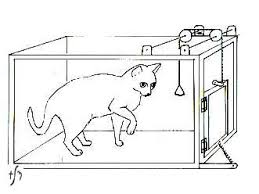
\includegraphics[scale=0.6]{slike/macka.jpg}
    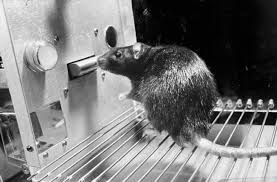
\includegraphics[scale=0.5]{slike/miska.jpg}
\end{frame}


\begin{frame}
    \frametitle{Spodbujevano učenje}
    \begin{itemize}
        \item \textbf{Okolje, agent, nagrada, (model)}
        \item Pomemben je čas
        \item Ne poznamo ">pravilnih"> akcij
        \item Raziskovanje in izkoriščanje
        \item Vrednostna funkcija
    \end{itemize}
\end{frame}


\begin{frame}
    \frametitle{Kje je to uporabno?}
    \begin{itemize}
        \item Naučiti robota hoje
        \item Upravljati s portfeljem
        \item Igrati namizne igre
        \item Igrati katerekoli igre
        \item ...
    \end{itemize}
    Torej res praktično karkoli, kjer lahko cilj modeliramo kot numerične
    nagrade, ne poznamo pa optimalnih akcij za dostop do teh nagrad.
\end{frame}


\begin{frame}
    \frametitle{Problem}
    Reward hypothesis
\end{frame}


\begin{frame}
    \frametitle{Primer: Križci in krožci 1}
    \begin{itemize}
        \item tu slika tistega loopa
        \item \textbf{Stanje:} Kje je prazno, kje ">X"< in kje ">O"<
        \item \textbf{Agent:} Program, ki se odloča, kako igrati
        \item \textbf{Okolje:} Agentu sporoča nagrade in stanje
        \item \textbf{Nagrada:} Pozitivna za zmago, negativna za poraz
    \end{itemize}
\end{frame}


\begin{frame}
    \frametitle{Primer: Križci in krožci 2}
    \begin{itemize}
        \item Agent igra igre, posodablja svoje vrednosti stanj glede na odgovor okolja
        \item Kako naj to stori?
    \end{itemize}
\end{frame}


\begin{frame}
    \frametitle{Primer: Križci in krožci 3}
    \begin{itemize}
        \item Enostavna ideja:                                  \pause
        %
        $$
        V(s) \leftarrow V(s) + \alpha [R + \gamma V(s') - V(s)]
        $$
        %
                                                                \pause
        \item \textit{s} je trenutno stanje                     \pause
        \item \textit{V} je vrednostna funkcija                 \pause
        \item $\alpha$ je velikost koraka (hitrost učenja)      \pause
        \item $\gamma$ je diskontni faktor (pomemben je čas)    \pause
        \item \textit{s'} je stanje, ki sledi \textit{s}        
    \end{itemize}
\end{frame}


\begin{frame}
    \frametitle{Bistvo}
    %
    $$
    \text{nova ocena} \leftarrow \text{stara ocena} + \text{korak} 
    [\text{cilj/tarča} - \text{stara ocena}]
    $$
    %
\end{frame}


\begin{frame}
    \frametitle{Kako lahko to posplošimo}
    \begin{itemize}
        \item Koliko stanj imamo?
        \item Do kje lahko pridemo?
        \item Kdaj odpove?
        \item Kaj je rešitev?
    \end{itemize}
\end{frame}


\begin{frame}
    \frametitle{Demonstracija: Križci in krožci}
    Morda kakšna slika/grafikon
\end{frame}


\end{document}
